% This file should be replaced with your file with an thesis content.
%=========================================================================
% Authors: Michal Bidlo, Bohuslav Křena, Jaroslav Dytrych, Petr Veigend and Adam Herout 2019

\hyphenation{OpenStack Swift OpenIO SDS}

\chapter{Introduction}

% general introduction for a topic:
%- cloud computing popularity
%- most popular service: cloud storage and its types
%- about object storage
%- users interest of what's going in theirs storage / event activities
%- TODO: maybe remove talk about types of cloud storages? solution: talk about need for monitoring and users need to monitor/receive information regarding their storage
In the current world, cloud computing became the most popular way of delivering different types of services throught Internet. One of the most popular cloud service is cloud storage, which allows users to store data in remote locations mentained by third party. Based on how cloud storage manages data, cloud storage can be divided into 3 types: Block storage, File storage and Object storage. Object storage manages data as objects, each object typically includes data itself and some additional informations stored in objects metadata. Since data are stored in remote locations, to which users don't have direct and complete access, some users or external services might want to receive informations about certain events (for example change of content) in storages where their data are located.

% importance of thesis in this field
%- react to events - possibly react to 'bad' events
%- allows users to have better picture what is going on in their storage
Importance of this thesis is to provide event informations to users in OpenIO SDS and OpenStack Swift, which will allow user to react on those events and possibly prevent/detect unwanted actions. Providing event notifications will allow users to have better picture on what is going on in their storage and impove monitoring in these object storages.

%past advances in this field
There was two attempts\cite{swiftPatch1}\cite{swiftPatch2} to solve this issue within OpenStack Swift which were not officially accepted and their solution is outdated. Currently there is no official solution for publishing event notification in OpenStack Swift nor OpenIO Software-Defined Storage (hereinafter SDS).

%why am I interested in this, why I choose this topic
%- perosnally i used object storage
%- can se myself using this solution in future as well as millions of other users
%- impact on big amount of users
%- contibuting to open source projects
My interest in this topic steems from its possible impact to extensive amount of users that OpenStack Swift and OpenIO have. Contibuting to open source projects is something that I always wanted to be part of. Possiblity to improve user experience in OpenStack Swift and OpenIO SDS and allow those storages to be even more competative against comercial storages (Amazon, Google, ...) is another reason why I choose this topic.

%goals of thesis
The goal of this thesis is to create program/middleware which wil publish event notification to user specified destination. One of supported destination will be Beanstalk queue, but program will allow to easily add other types of destinations (for example Kafka) using predefined interface. Proposed program will allow user to specify, using objects metadata (such as name prefix/sufix and object size) and type of event, which event notification should be published. Program will be able to run within OpenStack Swift as well as OpenIO SDS. This thesis will strive to find such solution that could be officially accpeted as part of OpenStack Swift and OpenIO SDS.

%structure of thesis
Structure of thesis - TODO - there will be probably change in chpaters structure

\chapter{Background}

This chapter introduces Object storage and its core concepts along with the underlying technologies. For sufficient understanding its important to explain how Software-defined storage manages data and what types of events can occur inside. The last part of this chapter describes concept of event notifications, why are they important and current interfaces for publishing event notifications to users.

\section{Object storage}
    %introduction/concept
    Object storage, also known as \textit{object-based storage} (OBS), is type of storage that handles data as objects, instead of hierarchical methods used in file systems\cite{objectBasedStorage}. Object stores are designed at handling data as whole objects, making them ideal solution for any unchanging data. Data in object stores are changed by replacing objects or files and therefore object stores are prefered mechanicsm for storing such files\cite{networkStorage}.

    %key koncepts
    %-metadata are stored in same object store device but on separated location
    \subsection{Key concepts}
    Key concepts of object storage are\cite{ibmObjectStorage}:
    \begin{itemize}
        \item{Objects - An object typically consist of user data and metadata uploaded to objected storage.}
        \item{Containers/Buckets - represents logical abstraction that is used to provide a data container in object storage. An object with same name in two different containers represents two different objects. This concept is used to segragate data using bucket ownership and a combination of public and secret keys bound to object store accounts which allows users and application to manipulate with data that are authorized for specific type of manipulation (read/write/update).}
        \item{Metadata - Additional information about data, create and last modified date, size, hash,...}
        \item{Access Control Lists(ACLs) - used as primary security construct in object storage, stored in account or bucket level and allows owners to grant permissions for certaint operations based on UUID, email, ...}
        \item{Object Data protection - two main schemes of data protections in object storage are \textbf{Replication} and \textbf{Erasure Coding}.

        Replication is method to ensure data resilience. Data are copied into multiple locations/disks/partitions, in case of failure, data are used from secondary copy, either to recreate original copy or as main copy.

        Erasure coding is process throught the data is separated into fragments. Then fragments are expanded and encoded with redundant pieces and stored across different storage devices. Erasure coding adds redundancy and allows object storage to tolerate failures.}
    \end{itemize}


    \subsection{Object data}
    %types of stored informations
    With object storage techniques, each object contains\cite{ibmObjectStorage}:
    \begin{itemize}
      \item{Data - user specified data that needs to be stored in persistent storage. It can be binary data, text file, image, etc..}
      \item{Metadata - Extra data describing objects data and can be divided into two types: Device-managed metadata is additional information maintained by storage device and used as part of object management in physical storage.\cite{objectBasedStorage}. Second type is Custom metadata, where user can store any additional information in key and value pairs. In object storage metadata are stored together with the object.}
      \item{A universally unique identifier (UUID) - This ID, created using hashing process based on object name and some other additional informations, is assigned to each object in a Object storage. Using ID object storage systems are cappable of tell a part objects from one another and ID is used to extract data in system without knowing their physical location/drive and offset.}
    \end{itemize}

    \subsection{Access to object storage}
    %access to object storage
    %-resfull interface
    %-advantages of this approach
    %-popular intefaces
    Obeject storage services provide RESTful interface \cite{cloudObjectStorage} over HTTP protocol for objects store and access. This approach allows users to create, read, delete, update or even query objects anytime and anywhere simply by referencing UUID (or using certain attributes for querying), usually with proper authentication process. Most popular interfaces for comunicating with object storages are Amazon S3 (Simple Storage Service) API and OpenStack Swift API.

    %comparison to other storage models
    \subsection{Pros and cons of object storage}
    Pros:
    \begin{itemize}
        \item{Cappable of handling large amount of unstructured data}
        \item{Reduced TCO and cheap COTS - Object storage is designed to utilize cheap COTS(Commercial off-the-shelf) components, as result Total Cost of Ownership(TCO) is lower then owning home-made Network-Attached Storages(NAS)\cite{networkStorage}.}
        \item{Unlimited scalability - Since object storages are build on distributed systems, they scale very well compared to traditional storages where they often have upper limit.\cite{openstackObjectStorage}}
        \item{Wide-open metadata - allows users to store custom metadata and posibility of createing metadata-driven policies, such as compression and tiering.}
    \end{itemize}
    Cons:
    \begin{itemize}
        \item{No in-place update - object must be manipulated as whole unit}
        \item{No locking mechanicsm - object storage does not manage object-level locking and it is up to applications to solve concurrent PUT/GET.}
        \item{Slower - this makes object storages poor choice for applications that need rapid and frequent acess to data.}
    \end{itemize}

\section{Software-Defined storage}
    %introduction to topic
    Software-Defined storage(SDS) is storage architecture which separates software storage from hardware allowing greater scalability, flexibility and control over data storage infrastructure.
    With growth of Software-Defined Networks(SDN) and need of Software-Defined Infrastructure(SDI), which aims to virtualize network resources and separate control plane from data plane, this principle was needed to be apply on Object storages as well\cite{sdsSDSMultiTenantEnv}.

    To overcome limitations of traditional storage infrastructures, the Software-Defined Storage (SDS) is imposed as proper solution to simplify data and configuration management, while improving end-to-end control functionality of conventional storage systems\cite{sdsSurvey}. While traditional storages like  storage area networks (SAN) and network-attached storage (NAS) provides scalability and reliability, SDS provides it with much lower cost by utilizing industry-standard or x86 system and therefore removing dependency on expensive hardware\cite{sdsWPRedHatSDS}.

    %principles
    % - Scale-out
    % - Customizable
    % - Automation
    % - Masking
    % - Policy Management
    \subsection{Principles}
    There is no clear definition on criteria for defining software-defined storage, although several key principles can be deducted\cite{sdsGPCloudStorage}:
    \begin{itemize}
        \item Scale-out - SDS should enable low-cost horizontal scaling (by adding new commodity hardware to existing infrastructure) compared to vertical scaling with more powerfull (and expensive) hardware.
        \item Customizable - SDS should offer system storage customization to meet specific storage QoS requirements. This will allow users to choose storage solution based on their requirements/performance and avoid unnecessary overpaying.
        \item Automation - once QoS is defined process of deployment and monitoring on object storage should be automated and done without need to human resources.
        \item Masking - SDS can mask underlying storage system and distributed system as lons as they provide common storage API and meet required QoS. For SDS can offer block or File API even though data are saved in object storage (like Ceph does).
        \item Police Management - SDS Software must manage storage according to specified policies and QoS requirements despite being in multi-tenant space. SDS must be cappable to handle failures and autoscale in case of change in workloads.
    \end{itemize}


    %architecture
    %   - data plane
    %   - control plane
    %functions
    %benefits
    \subsection{Architecture}
    As previously described, the main characteristic of SDS is to separate storage functions into control plane and data plane.

    \paragraph{Control plane}
    - the control plane represents an abstraction layer with main goal to virtualize storage resources. It offers high-level functions that are needed by the customer to run the business workload and enable optimized, flexible, scalable, and rapid provisioning storage infrastructure capacity. These capabilities span functions like policy automation, analytics and optimization, backup and copy management, security, and integration with the API services, including other cloud provider services\cite{sdsIBMSDSGuide}.

    \paragraph{Data plane}
    - the data plane encompasses the infrastructure where data is processed. It consists of all basic storage management functions, such as virtualization, RAID protection, tiering, copy services (remote, local, synchronous, asynchronous, and point-in-time), encryption, compression, and data deduplication that can be requested by the control plane. The data plane is the interface to the hardware infrastructure where the data is stored. It provides a complete range of data access possibilities and spans traditional access methods, such as block I/O (for example, iSCSI), File I/O (NFS, SMB, or Hadoop Distributed File System (HFDS)), and object-storage\cite{sdsIBMSDSGuide}.

    %todo image of layers from sdsSurvey
    \begin{figure}[hbt]
        \centering
        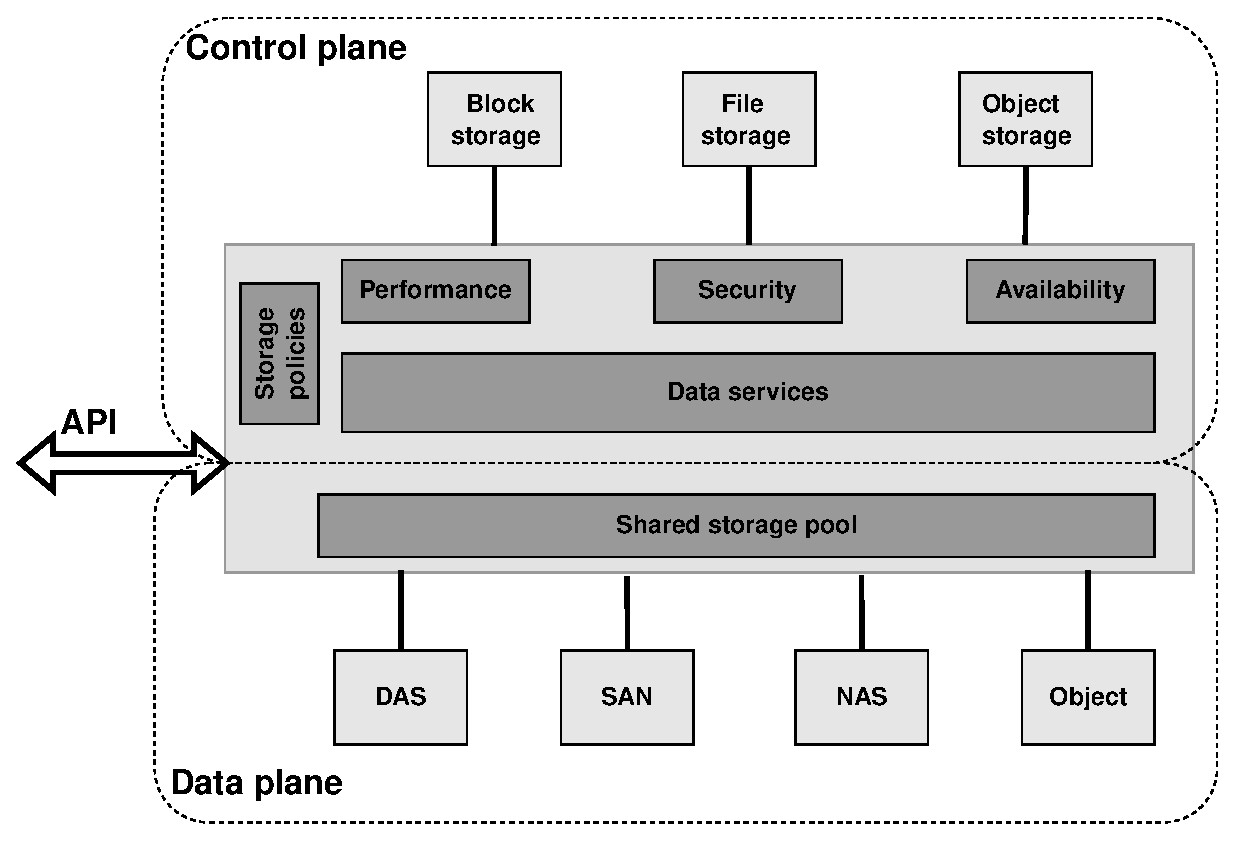
\includegraphics[width=1\textwidth]{obrazky-figures/sds-planes.eps}
        \caption{SDS data and control plane.\cite{sdsPlanes}, remade}
        \label{fig:beanstalkdJobSM}
    \end{figure}

\section{Beanstalk queue}

    Beanstalk queue or shorter beanstalkd is fast, simple and lighweight working queue\cite{}. Main use case is to manage workflow between different parts of workers of application throught working queues and messages. Beanstalkd was developed for need of Facebook application in order to reduce average response time\cite{beanstalkdOfficial}. Provided by simple protocol design, heavily inspired by memcached, implemented in programming language C, Beanstalkd offers lean architecture which allows it to be installed and used very simply, making it perfect for many use cases\cite{beanstalkdInstall}.


    \subsection{Beanstalkd elements}
    Beanstalkd is priority queue with server-client architecture. Server represents queues where jobs are saved based on priority. Beanstalkd architecture is composed from several components:
    \begin{itemize}
        \item Jobs - tasks stored by client
        \item Tubes - used for storing tasks, each tube contains a ready queue and a delay queue.
        \item Producer - create and send jobs to beanstalkd using command "put"
        \item Consumer - process "listening" on assigned tube, reserves and consumes jobs from tube
    \end{itemize}

    \subsection{Job Lifecycle}
    Each job is uniquely assigned to one worker at a time. A job in beanstalkd is created by client using "put" command. While being in tube, job can be in next states\cite{beanstalkdProtocol}:
    \begin{itemize}
        \item READY - the task is free and can be executed immediately by consumer.
        \item DELAYED - the task has assigned delay time that needs to expire before execution. After delay time expires, beanstalkd will automaticly change it state to READY.
        \item RESERVED - the task is reserved and is being executed by consumer. Beanstalkd is responsible for checking whether the task is completed in time (TTR - Time to run).
        \item BURIED - reserved task, the task will not be removed nor executed until client decides. This state is often used for futher inspection in debug process when failure or undefined behavior occurs during task execution.
        \item DELETED - the task is deleted from tube, beanstalkd no longer maintains these jobs.
    \end{itemize}

    Figure \ref{fig:beanstalkdJobSM} describes life cycle of job in beanstalkd tube. Job is created by Producer using put command. Beanstalkd allows Producer to add delay time before task will be ready for execution, which sets job state to DELAYED. After delay time expires, beanstalkd will automaticly change job state to READY. Producer can specify job priority and jobs with READY state are stored in priority queue. Job with biggest priority is reserved and executed by Consumer. After succesfully executing the task, Consumer will delete job from beanstalkd. If some error occured, Consumer can burry the task. Consumer can decide that is not interested in compliting reserved task. Using release command (with optional delay) job state will be changed back to READY (or DELAY).
    Jobs with BURRIED state will not be touch by beanstalkd server until client "kicks" them to READY state.

    \begin{figure}[hbt]
        \centering
        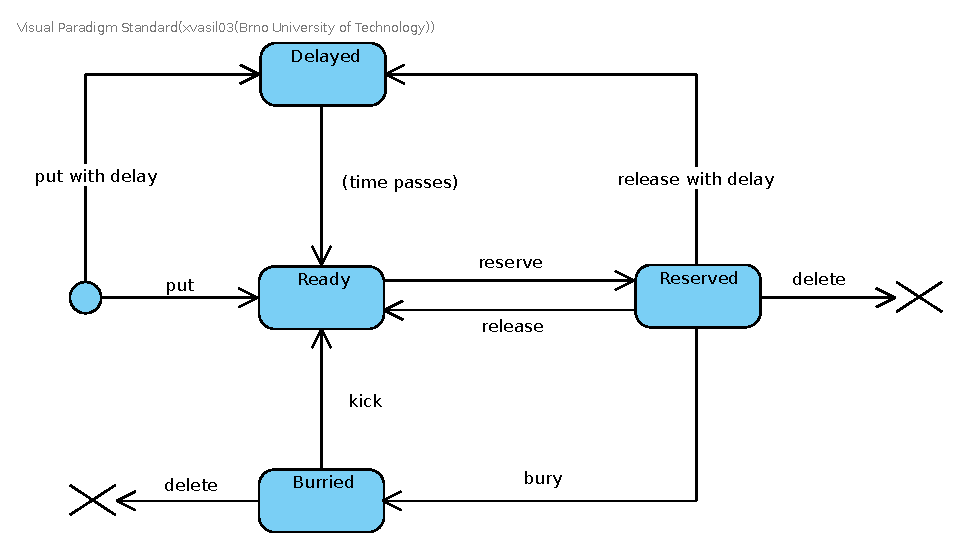
\includegraphics[width=1\textwidth]{obrazky-figures/beanstalkd-job-states.eps}
        \caption{State machine diagram of job in Beanstalkd tube}
        \label{fig:beanstalkdJobSM}
    \end{figure}


    \subsection{Key characteristics}
    Key beanstalkd characteristics are:
    \begin{itemize}
        \item Asynchronous - beanstalkd allows producers to put jobs in queue and workers can process them later.
        \item Distributed - in a same way as memchaced, beanstalkd can be distributed although this distribution is handled by clients. The beanstalkd server doesn't know anything about other beanstalkd instances that are running.
        \item Persistent - beanstalkd offeres support for persistent jobs durring which all jobs are written to binlog. In case of power outrage, after restarting beanstalkd instance will recover jobs content from the logs.
        \item Not secured - beanstalkd is designed to be runned in private/secured network. Therefore it does not support authentication nor authorization.
        \item Scalability - beanstalkd can be scaled horizontally, although it must be done on client side, where each client would connect to multiple servers and then use specific algorithms(e.g. Round-robin) to switch between the different servers.
    \end{itemize}

\section{Event notifications}
    %introduction
    An event is a runtime operation, executed by a software element, representing significant change or occurence in system. Event is created in order to make some information avaliable to other software elements not specified by the operation\cite{eventArchitecturalPatterns}.

    Event notification is a message, created by system in order to inform other to notify other parts of system that an event has taken place\cite{eventRedHatEventDrivenArch}. Event notifications are used for monitoring and asynchronous job processing.

    In object storage, event notifications are used as mean to notify users or tenants about specific changes and occurences in their bucket or account. Typical event notifications are regarding creating new (or updating existing) objects in bucket. Most object vendors offers Publish/subscribe notifications, which allows users to subscribe to certain type of event notifications using predefined types of rules. Informations about rules specifiying event notifications are usually stored in metadata of upper level (bucket or account).

    \subsection{CloudEvents}
    Publishers tend to desribe event data differently due non existing standard or format. The lack of common way to describe events means that developers have to learn how handle events for each event source. To solve this problem CloudEvents was created.

    CloudEvents is a specification for describing event data in common way\cite{eventCloudEvents} hosted by Cloud Native Computing Foundation (CNCF)\cite{eventCNCF}. CloudEvents goal is to dramatically simplify event specification and delivery across services, platform and beyond.
    CloudEvents has been integrated by many popular object storage vendors, such as Oracle Cloud, IBM Cloud Code Engine, Azure, Google Cloud etc.

    \paragraph{Specification}
    Attributes in CloudEvents specification can be divided into 3 categories.

    REQUIRED Attributes - set of attibures that are required to be included in all events\cite{eventCloudEventsSpec}:
    \begin{itemize}
        \item id (string) - event identifier, must not be empty.
        \item source (URI-reference) - identifies context in which event occured, must not be empty.
        \item specversion (string) - the version of CloudEvents specification, must not be empty.
        \item type (string) - value describing type of occured event. Often this attribute is used for policy enforcment, routing and monitoring.
    \end{itemize}

    Event data attirbutes are attibures containing and describing event data:
    \begin{itemize}
        \item datacontenttype (string) - content type of data value (allows data to carry any type of content).
        \item dataschema (URI) - identifies the schema that data adheres to.
        \item data - data payload
    \end{itemize}

    OPTIONAL attibutes:
    \begin{itemize}
        \item time - timestamp
        \item subject (string) - the subject of the event in the context of the event producer.
        \item extension attributes - custom attibutes allowing external systems to attach metadata to an event.
    \end{itemize}

    \definecolor{darkpastelred}{rgb}{0.76, 0.23, 0.13}
    \lstset{
        string=[s]{"}{"},
        stringstyle=\color{darkpastelred},
        comment=[l]{:},
        commentstyle=\color{black},
    }
    Example:
    \begin{lstlisting}
    {
        "specversion" : "1.0",
        "type" : "com.github.pull_request.opened",
        "source" : "https://github.com/cloudevents/spec/pull",
        "subject" : "123",
        "id" : "A234-1234-1234",
        "time" : "2018-04-05T17:31:00Z",
        "comexampleextension1" : "value",
        "comexampleothervalue" : 5,
        "datacontenttype" : "text/xml",
        "data" : "<much wow=\"xml\"/>"
    }
    \end{lstlisting}

    \subsection{Amazon S3 event notifications}
     Amazon Simple Storage Service (S3) is one of the most popular cloud object storages providing REST web service interface. Amazon S3 is reliable, scalable and commercial object storage that manages Web-Scale computing by itself\cite{eventS3}. Amazon S3 had big impact on object storage and most of other object storage vendors crated compatible S3 API for their services.

     One of the monitoring features that Amazon S3 provides is Event Notification, feature offering users to receive notifications when certain event happens in their S3 bucket. To enable such notifications, users needs to create notification configuration that identifies witch events Amazon S3 should publish\cite{eventS3EventNotification}. Notifications are configured at the bucket level and then applied to each object in the bucket.

     Amazon S3 provides limited event destinations to which event notification messages can be send\cite{eventS3EventNotificationDest}:
     \begin{itemize}
         \item Amazon Simple Notification Service (Amazon SNS) - flexible, fully managed push messaging service, can be used to send messages to mobile phones or distributed services.
         \item Amazon Simple Queue Service (Amazon SQS) queues - reliable and scalable hosted queues for storing messages as they travel between computers.
         \item AWS Lambda - serverless, event-driven compute service. Lambda can run custom code in response to Amazon S3 bucket event (if lambda function writes to same bucket that triggers the notification, it can create an execution loop).
         \item Amazon EventBridge - serverless event bus used for receiving events from AWS. It allows users to define rules to match events and deliver them to defined targets.
     \end{itemize}

     By this date, Amazon S3 does not support CloudEvents specification and describes event data in their own way. Some of event types that Amazon S3 can publish are\cite{eventS3EventNotificationDest}:


     \renewcommand*{\arraystretch}{1.4}
     \begin{tabularx}{\textwidth}{|p{0.3\textwidth}|X|}
         \hline
         \textbf{Event type} & \textbf{Desription} \\
         \hline
         s3:TestEvent & after enabling the event notifications, Amazon S3 publishes a test notification to ensure that topic exist and bucket owner has permissions to publish specified topic. \\
         \hline
         s3:ObjectCreated:* & An object was created (regardless on operation). \\
         \hline
         s3:ObjectCreated:Put & An object was created by an HTTP PUT operation. \\
         \hline
         s3:ObjectCreated:Post & An object was created by HTTP POST operation. \\
         \hline
         s3:ObjectCreated:Copy & An object was created an S3 copy operation. \\
         \hline
         s3:ObjectCreated:

         CompleteMultipartUpload & An object was created by the completion of a S3 multi-part upload. \\
         \hline
         s3:ObjectRemoved:* & An object was removed (regardless on operation). \\
         \hline
         s3:ObjectRemoved:Delete & An object was deleted by HTTP DELETE operation. \\
         \hline
         s3:ObjectRemoved:

         DeleteMarkerCreated & An versioned object was marked for deletion. \\
         \hline
    \end{tabularx}


\chapter{OpenIO SDS}
    OpenIO Software-defined storage is open source object storage that is perfectly cappable of traditional use cases (such as archiving, big data, cloud) but at same time, combining with Grid for Apps (\ref{sec:oioGridForApps}), it opens the door for users to create application that need much more sofisticated back-end operations. These applications includes industrial IoT, machine learning and artificial intelligence, as well as any other applications whose workflow can benefit from automated jobs or tasks\cite{oioNextGen}. OpenIO SDS is event-driven storage with ability to itercept events seamlessly and transparently to the rest of the stack.

    \section{Key characteristics}
    \subsection*{Hardware agnostic}
    OpenIO SDS is fully software-defined storage cappable of running on x86 or ARM hardware with minimal requirements. Cluster nodes can be different from each other, allowing different generations, types and capacities to be combined without affecting a performance or efficiency\cite{oioKeyChars}.
    OpenIO has built-in support for heterogeneous hardware allowing every node to be used at its matixmum performance.
    \subsection*{No SPOF architecture}
    Every single service used to serve data is redundant. From object chunks stored in disck, to directory level, every information is duplicated. As a result there is no single point of failure (SPOF) in cluster and node can be shutdown without affecting overal avaliability or integrity\cite{oioCoreSolution}.
    \subsection*{Cluster organization}
    Instead of traditional cluser ring-like layout, OpenIO SDS is based on grid of nodes \ref{fig:oioArch}. It is flexible and resource conscious. Compared to other object storage solutions, cluster organization is not based on static data allocation that usually use Chord peer-to-peer distributed hash table aglorithm. Instead OpenIO SDS uses distributed directory for organizing data and metadata hash tables, whcih allows the software to attain same level of scalability but with better and more consistent performance\cite{oioKeyChars}.

    \begin{figure}[hbt]
        \centering
        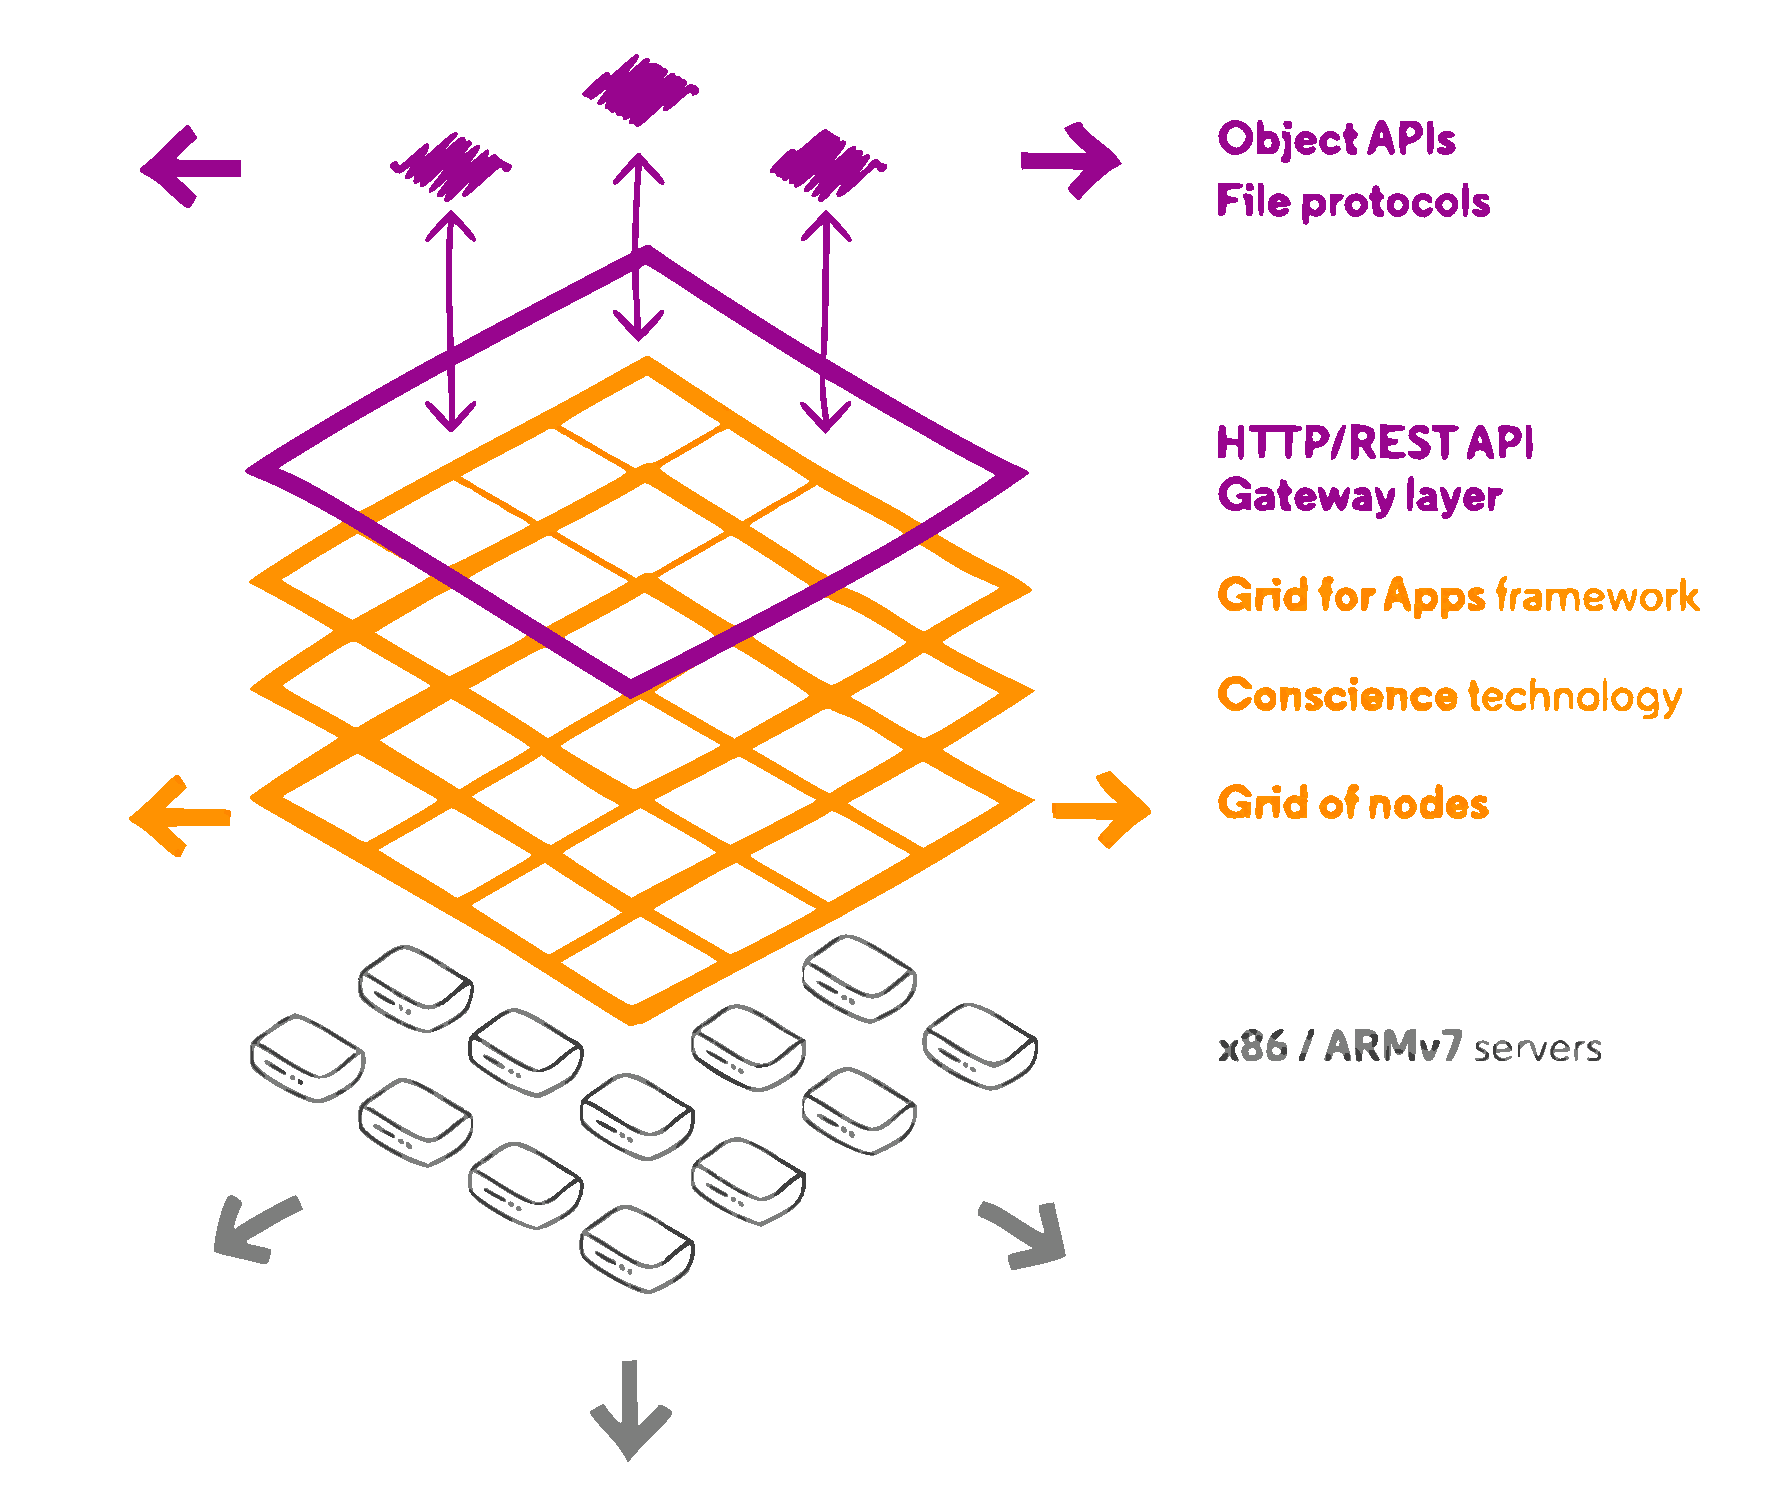
\includegraphics[width=1\textwidth]{obrazky-figures/openio-architecture.eps}
        \caption{Layered view on OpenIO SDS architecture.\cite{oioArch}}
        \label{fig:oioArch}
    \end{figure}


    \subsection*{Tiering}
    With tiering, OpenIO SDS offers users to configure pool containing group of hardware which then can be used for storing specific types of objects. For example, user can create pool of high performance hard disks (e.g. SSDs) and use the pool for storing objects that require low latency.
    This feature is realised by mechanism called storage policies. Multiple storage policies can be defined in one particual namespace. Storage policies can also be used for specifying how many replicas should be created for specific dataset\cite{oioCoreSolution}.

    \section{Data organization}
    Multi-tenancy is one of the core concepts in OpenIO SDS. Data objects are stored within following hierarchy: Namespace/Account/Container/Object \ref{fig:oioDataOrganization}. Multiple namespaces can be configured in each cluster, providing multi-region/zone logical layouts for applications and segregated workloads depending on a tenant or geo-distribution need\cite{oioSdsConcepts}.
    There is no classic subdirectory tree. Object are stored in flat structure in container level. Like many other object storages, there is a way to simulate filesystem.

    \begin{figure}[hbt]
        \centering
        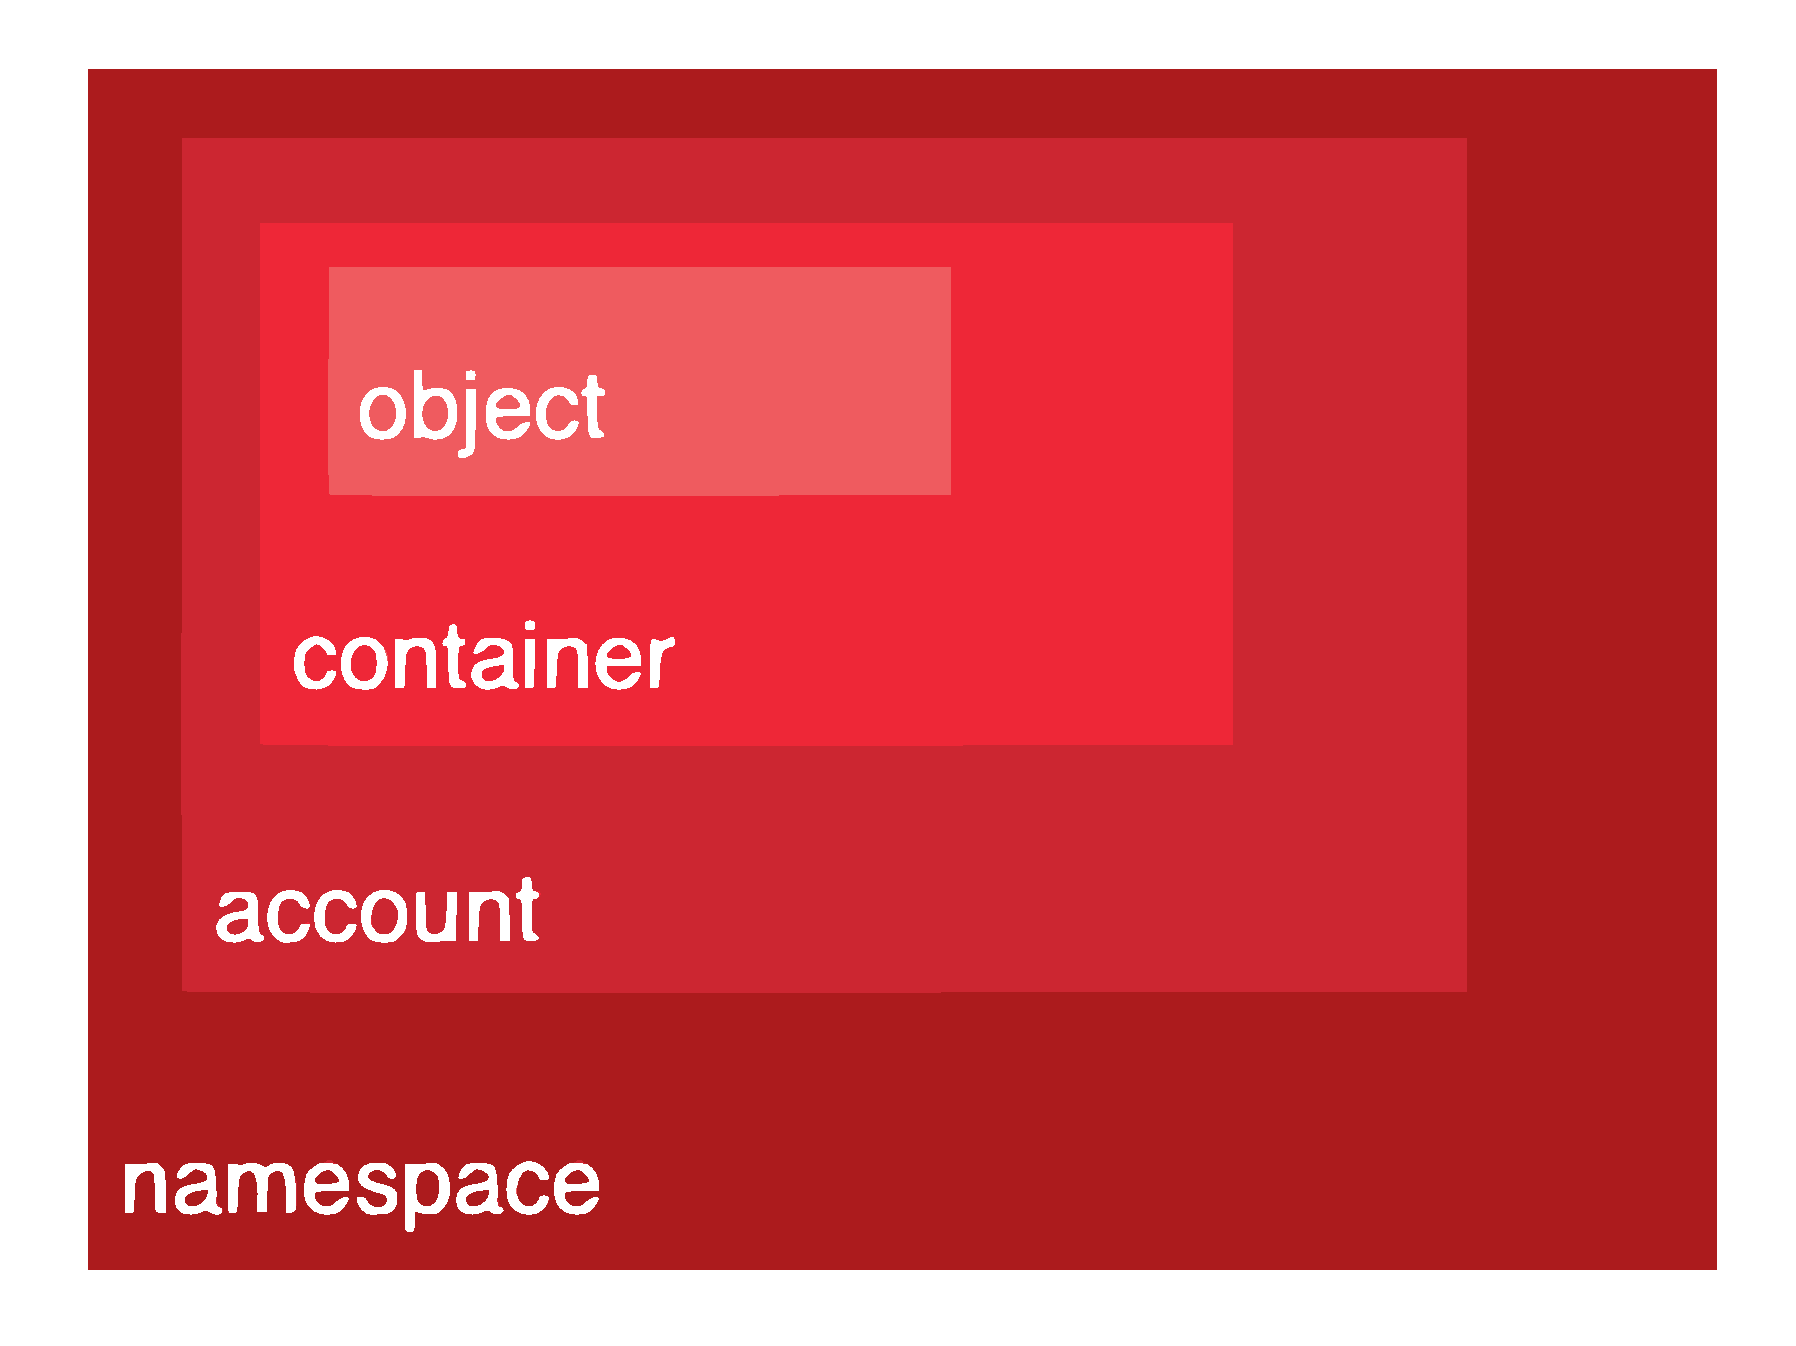
\includegraphics[width=0.5\textwidth]{obrazky-figures/openio-data-organization.eps}
        \caption{Object data organization in OpenIO SDS.\cite{oioArch}}
        \label{fig:oioDataOrganization}
    \end{figure}

    \subsection{Namespace}
    A coherent set of network services working together to run OpenIO’s solutions. It hosts services and provides operations such as service configuration and monitoring.

    \subsection{Account}
    An account usually represents a tenant and is the top level of data organisation. Each account owns and manages a collection of containers. Accoun keep track of namespace usage for each customer (i.e. bytes occupied by all of a customer's objects)\cite{oioCoreSolution}.

    \subsection{Container}
    Container represents a object bucket. Each container belogs to one (and only one) account and is identified by a name which is unique within the account. The contaier carries additional information specifiying how to manages its objects (e.g. how to secure them)\cite{oioCoreSolution}.

    \subsection{Object}
    Object is the smalles data unit visiable by customer and represents a named BLOB with metadata. OpenIO SDS allows several objects to be stored in a container, and are considered as versions of same object. Classic API operations (PUT/GET/DELETE) will be directed towards object with latest version. If size of object is higher then specified limit at the namespace level, the object will be divided into chunks of data. This allows capacity optimalization as well as distributed reads that could be particularly useful for high-speed video streaming of large medias for instance\cite{oioCoreSolution}.

    %\section{Services} maybe include?
    \section{Serverless computing}
    %what is serverless computing
    \subsection{Grid For Apps}\label{sec:oioGridForApps}

    Similarly to Amazon AWS Lambda, OpenIO offers event-driven compute service called Grid for Apps that works on top of OpenIO.

    Grif for Apps intercepts all the events that happen in the storage layer, and based on user configuration, triggers specific application or script to act on data (metadata) stored in object storage\cite{oioNextGen}. The application is executed in cluster nodes and utilizes free unused resources avaliable in the cluster. This impove efficiency (less data moving, since object data are already avaliable), and saves money (no need for external resources)\cite{oioNextGen}.

    Grid for Apps allows customers to perform operations such as metadata enrichment, data indexing and search (e.g. indexing metadata to Elasticsearch), pattern recognition, machine learning, data filterning, monitoring, etc\cite{oioNextGen}.

    Grid for Apps in OpenIO is realised using service event-agent and beanstalkd queue.

    \subsection{Event-agent}
    Event-agent is OpenIO service responsible for handling asynchronous jobs. It relies on beanstalkd backend to manages jobs. Event-agent key characteristics are\cite{oioSdsServices}:
    \begin{itemize}
        \item Stateless
        \item CPU intensive
        \item Must be deployed on ever server of the cluster
    \end{itemize}

    Every event that occurs in OpenIO is inserted in beanstalkd tube. Event-agent is listening the beanstalkd tube and consumes jobs from it. Consumers are produced using Eventlet Network Library \cite{oioEventlet}. Number or workers can be configured.

    In event-agent, user can specify handlers for each type of events in event-handler.conf.
    Some of the event types in OpenIO are storage.content.new, storage.container.deleted, etc.

    Events handler is defined as pipeline containing applications that will react to the event. For example, deleting an object will invoke storage.content.deleted event. Event-agent will handle the event using content\_cleaner application, which in fact deletes objects chunks from object storage.

    \begin{lstlisting}
    [handler:storage.content.deleted]
    pipeline = content_cleaner

    [handler:storage.content.new]
    pipeline = notify

    [filter:content_cleaner]
    use = egg:oio#content_cleaner

    [filter:notify]
    use = egg:oio#notify
    tube = oio-rebuild
    queue_url = ${QUEUE_URL}
    \end{lstlisting}
    %todo caption

    OpenIO offers users to process events outside of event-agent. In order to do that, user can use application "notify", which will simply send event to specified beanstalkd tube. After that user can create custom Consumer that will process the job from beanstalkd tube.

\chapter{OpenStack Swift}
\chapter{MinIO}

\chapter{Solution draft}
\section{Current state}
\section{Middleware for OpenStack Swift and OpenIO SDS}
\section{Adapter for MinIO}
\chapter{Implementation, experiments and assessment}

\chapter{Conclusion}

%=========================================================================
